\documentclass [12pt] {article}
\usepackage{graphicx, amsmath, amssymb}

\begin{document}

\title{Homework 0}
\author {Zach Stecher}
\date{Due: 9/6/16}
\maketitle

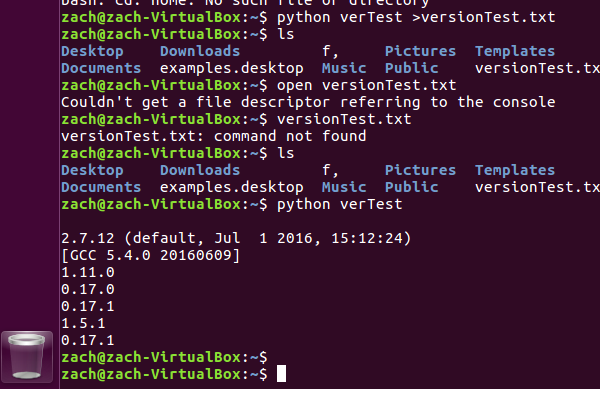
\includegraphics{ScreenShot}
Screenshot of Python package verion test. The output is also hosted on GitHub.


\includegraphics{Collab}
Screenshot of Professor Rivas added as GitHub Collaborator.\\
Username: zachstecher\\
Link: https://github.com/zachstecher/MSCS550

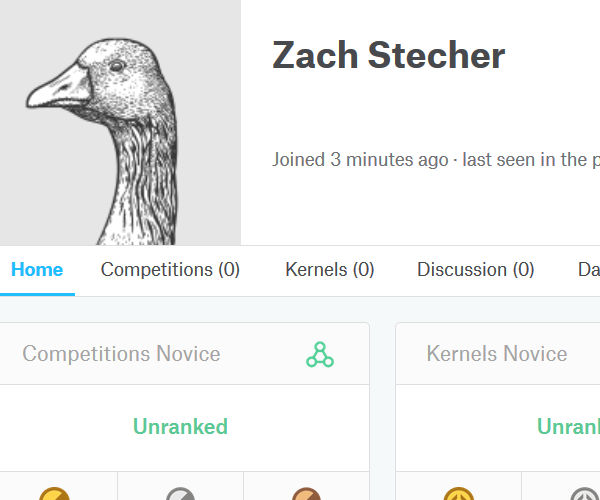
\includegraphics{kaggle}
Screenshot of kaggle account created with marist e-mail address.\\
Username: zstecher\\
Link: https://www.kaggle.com/zstecher
\newpage

Problems:\\
\\
1) Find the value for $x$ that maximizes g($x$).

Using \( \frac{-b}{2a} \) we compute that $x$ = 4 will maximize g($x$).

$x$ = 4\\
\\
2) What are the partial derivatives of f($x$) with respect to $x_0$ and $x_1$?

With respect to $x_0$: 9$x_0^2$ - 2$x_1^2$

With respect to $x_1$: -4$x_0x_1$ + 4\\
\\
3) Questions about given matrices:

a) Can you multiply the two matrices?\\
No. The number of rows from martix A do not match the number of rows from matrix B.\\

b)Multiply A\textsuperscript{T} x B and give its Rank:\\

\[
	C=
	\begin{bmatrix}
	-2 & -2 & 13 \\ 
	-8 & 1 & 16 \\ 
	6 & -3 & -3		
	\end{bmatrix}
\]

Matrix C has a Rank of 2.\\

c) $AB\textsuperscript{T}$ + $C^-1$ =\\

\[
	\begin{bmatrix}
	-16 & -16 \\
	11 & 13.5
	\end{bmatrix}
\]\\
\\
4) Give the mathematical definitions of the simple Gaussian, multivariate Gaussian, Bernoulli, binomial, and exponential distribution.\\

simple Gaussian: 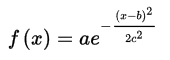
\includegraphics{Gaussian}\\

multivariate Gaussian:\\
 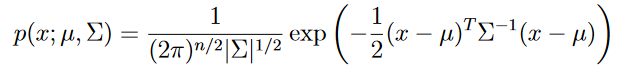
\includegraphics{multiGaussian}\\

Bernoulli: $P$($n$) = $P^n$(1 - $p$)\textsuperscript{1-$n$}\\

binomial: 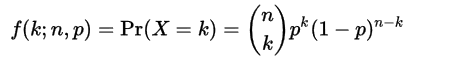
\includegraphics{binomial}\\

exponential: 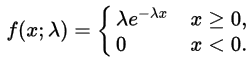
\includegraphics{exponential}\\
\\

5) What is the relationship between the Bernoulli and binomial distributions?\\

A Bernoulli distribution is a when a random variable $X$ has two possible outcomes: 0 and 1. A binomial distribution is when we take the sum of n independant Bernoulli random variables.\\
\\
6) The expected value is 2.5.\\
\\
7)Answer a) and b) for the given optimization problem.\\

a) $x$* = 1\\

b) Locate $x$* in the picture (added location):\\

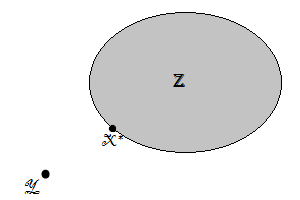
\includegraphics{Euclidean}\\

8) Couldn't figure out these problems in time...



\end{document}